\chapter{\label{ch:1-intro}Introduction} 

\graphicspath{{figures/ch1/}}

\minitoc

\section{General introduction}

\section{Structure and function of the pancreatic K\textsubscript{ATP} channel}

\subsection{Pancreatic islets and the \textgreek{b}-cell}

Pancreatic islets are endocrine cells which are responsible for maintaining glucose homeostasis.
There are roughly one million islets in a human pancreas, constituting 1-2\% of the total pancreatic mass.
Islets consist of three principal cell types; insulin secreting \textgreek{b}-cells, glucagon secreting \textgreek{a}-cells and somatostatin secreting \textgreek{d}-cells.
Islets respond to increases in blood glucose by releasing insulin, which acts on peripheral tissues to increase glucose uptake and reduce blood glucose levels.
Conversely, decreases in blood glucose leads to the release of glucagon, which acts on those tissues to stimulate glucose production and increase blood glucose.

\subsection{Glucose induced insulin secretion in \textgreek{b}-cells}

\subsection{Architecture of the pancreatic K\textsubscript{ATP} channel}

ATP-sensitive potassium (K\textsubscript{ATP}) channels are present in many tissues, where they couple the metabolic state of a cell to its electrical activity by regulating the flow of K\textsuperscript{+} across the membrane.
K\textsubscript{ATP} channels are an octameric complex, comprised of four inwardly-rectifying potassium channel subunits (Kir6.1 or Kir6.2), each of which is associated with a sulphonylurea receptor subunit (SUR1, SUR2A or SUR2B).
In pancreatic \textgreek{b}-cells, the K\textsubscript{ATP} channel isoform is composed of Kir6.2 and SUR1.

Inwardly-rectifying potassium channels are so named because they allow K\textsuperscript{+} to flow more easily into the cell than out of it (Figure \ref{ch1fig:rectification}).
This phenomenon is a consequence of voltage-dependent pore blockade by intracellular divalent cations (especially Mg\textsuperscript{2+}) and polyamines.
At depolarising membrane potentials, blockers are driven into the pore and K\textsuperscript{+} current is blocked, while at hyperpolarising potentials the blockers and cleared and K\textsuperscript{+} current can flow.
Strongly rectifying Kir channels display drastically reduced conductance at potentials more positive than the K\textsuperscript{+} reversal potential.
In contrast, Kir6.2 is a weak rectifier, and allows substantial current to flow at more positive potentials.

In addition to voltage, Kir6.2 is regulated by two endogenous ligands; 
phosphatidylinositol 4,5-bisphosphate (PIP\textsubscript{2}) and adenine nucleotides (Figure \ref{ch1fig:kir_struct}).
The binding of adenine nucleotides to Kir6.2 leads to closure of the channel pore, while the binding of PIP2 promotes the opening of the pore (Figure \ref{ch1fig:shyng_trace}).
Activation by PIP\textsubscript{2} is a mechanism common to the whole Kir family, wherease inhibition by nucleotides is unique to the Kir6 subfamily.

\begin{figure}[h]
	\centering
	\begin{subfigure}[t]{0.5\textwidth}
		\caption{}\label{ch1fig:rectification}
		\centering
		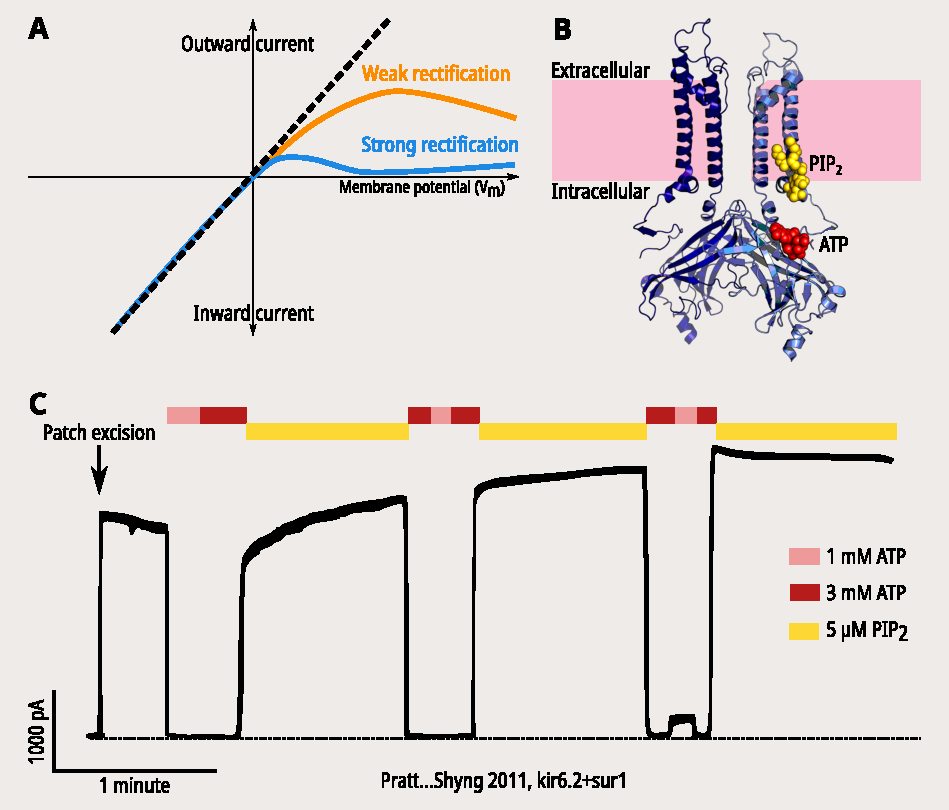
\includegraphics[width=\textwidth]{rectification.pdf}
	\end{subfigure}
	\hfill
	\begin{subfigure}[t]{0.4\textwidth}
		\caption{}\label{ch1fig:kir_struct}
		\centering
		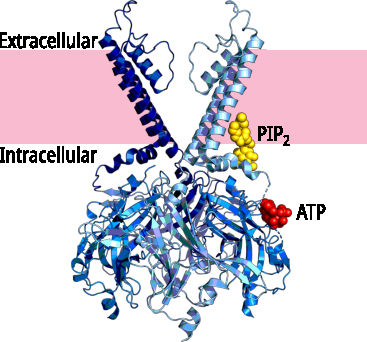
\includegraphics[width=\textwidth]{kir_structure.pdf}
	\end{subfigure}
	\vfill
	\begin{subfigure}[t]{0.9\textwidth}
		\caption{}\label{ch1fig:shyng_trace}
		\centering
		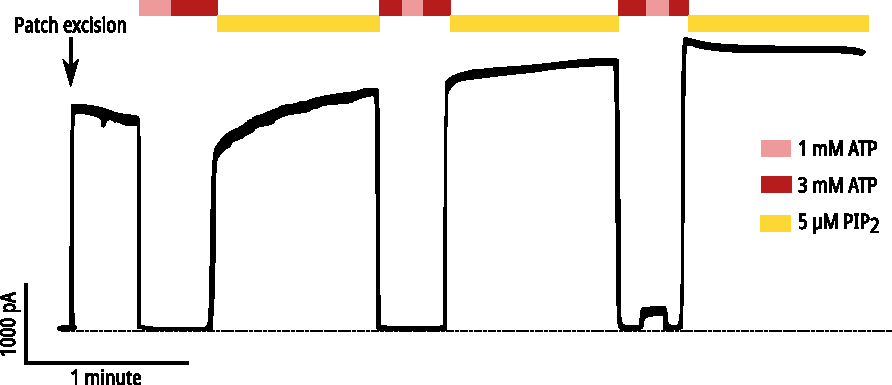
\includegraphics[width=\textwidth]{shyng_atp_pip_trace.pdf}
	\end{subfigure}
	\caption[Structure of Kir6.2]{
		\subref{ch1fig:rectification} Current-voltage plot demonstrating inward rectification of Kir channels.
		Here, the reversal potential of potassium (\textit{E\textsubscript{K}}) is set to zero, i.e. there is an equal concentration of K\textsuperscript{+} on each side of the membrane.
		Weak rectifiers such as Kir6.2 exhibit only a weak voltage dependent decline in conductance (visualised as a departure from the dashed line of an ideal conductor).
		(Kind of adapted from Handbook of Ion Channels).
		\subref{ch1fig:kir_struct} Cryo-EM structure of Kir6.2 (PDB \#6BAA) captured with ATP bound (red) and with the proposed binding position of PIP\textsubscript{2} visualised by alignment of the channel with the X-ray structure of Kir2.2 solved in compex with a short-chain dioctanoyl (diC8) PIP\textsubscript{2} (PDB \#6C3I).
		The plasma membrane is shown in pink.
		(Kind of adapted from Mike's JGP review).
		\subref{ch1fig:shyng_trace} Macroscopic currents from Kir6.2 channels coexpressed with SUR1 in excised patches from cultured cells, adapted from (Pratt/Shyng, 2011).
		Perfusion of ATP or PIP\textsubscript{2} is indicated by coloured bars, and demonstrates the contrasting effects of these two ligands on channel activity.
	}
	\label{ch1fig:kir_breakdown}
\end{figure}

SUR1 is a member of the ATP-binding cassette (ABC) family of transporters.
While other ABC proteins transport substrate across the membrane, SUR1 does not appear to do so; instead it acts to modulate the function of its associated ion channel.
The cystic fibrosis transmembrane conductance regulator (CFTR) is another member of the ABC family, and is an ion channel in its own right, capable of conducting chloride across the membrane.
Like other ABC proteins, SUR1 contains two sets of transmembrane domains (TMD1 and TMD2) and two cytosolic nucleotide binding domains (NBD1 and NBD2).
Unique to SUR is the presence of an additional transmembrane domain (TMD0) N-terminal to the core of the protein, and this domain forms the primary contact between SUR1 and Kir6.2.

The NBDs of ABC transporters are highly conserved, and consist of two subdomains: a larger RecA-like subdomain found in other P-loop ATPases, and a smaller \textgreek{a}-helical subdomain which is unique to ABC transporters.
There are three key structural motifs present in these subdomains: the RecA-like subdomain contains the Walker A (W\textsubscript{A}) and B (W\textsubscript{B}) motifs, while the \textgreek{a}-helical subdomain contains the ABC signature motif (typically LSGGQ).

The two domains come together to form an antiparallel dimer with two nucleotide binding sites (NBS1 and NBS2) at the interface, such that NBS1 is formed from the W\textsubscript{A} and W\textsubscript{B} motifs of NBD1 and the signature motif from NBD2, whereas NBS2 is formed from the W\textsubscript{A} and W\textsubscript{B} motifs of NBD2 and the signature motif from NBD1.
NBS2, also known as the consensus site as it is more similar in sequence to other ABC family members, is catalytically competent and able to hydrolyse ATP.
In contrast, NBS1 is the degenerate site, with a less conserved sequence and an inability to catalyse hydrolysis of ATP.

\begin{figure}[h]
	\centering
	\begin{subfigure}[t]{0.4\textwidth}
		\caption{}\label{ch1fig:sur_struct}
		\centering
		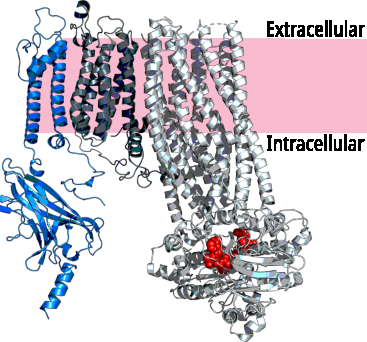
\includegraphics[width=\textwidth]{sur_structure.pdf}
	\end{subfigure}
	\hfill
	\begin{subfigure}[t]{0.5\textwidth}
		\caption{}\label{ch1fig:nbd_struct}
		\centering
		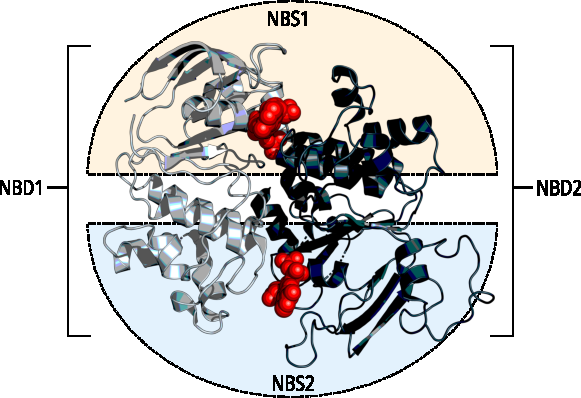
\includegraphics[width=\textwidth]{nbd_structure.pdf}
	\end{subfigure}
	\caption[Structure of SUR1]{
		\subref{ch1fig:sur_struct} Cryo-EM structure of SUR1 captured with a nucleotide (shown in red) bound at each NBS (PDB \#6C3P).
		A single SUR1 subunit is shown, with TMD1 and TMD2 in white and TMD0 in grey.
		A single Kir6.2 subunit is also shown in blue to show the interface between subunits.
		The plasma membrane is displayed in pink.
		\subref{ch1fig:nbd_struct} Top-down view of the NBDs from the same cryo-EM structure.
		NBD1 is on the left in white, NBD2 is on the right in grey, and the two NBSs are higlighted; NBS1 in orange and NBS2 in blue.
		Adapted from Mikes JGP review.
	}
\end{figure}

\subsection{Nucleotide regulation of the pancreatic K\textsubscript{ATP} channel}

\begin{figure}[h]
	\centering
	\begin{subfigure}[t]{0.9\textwidth}
		\caption{}\label{ch1fig:katp_cartoon}
		\centering
		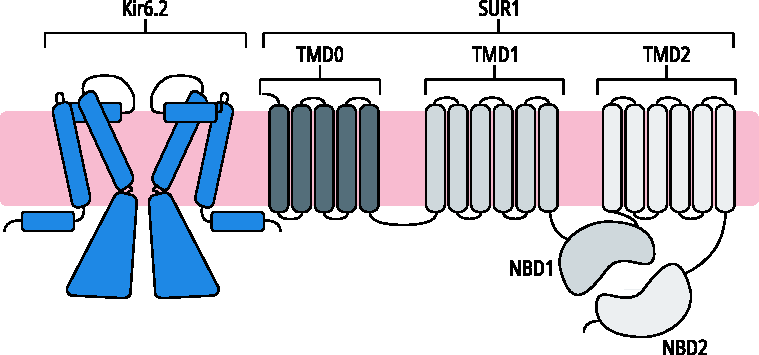
\includegraphics[width=\textwidth]{katp_cartoon.pdf}
	\end{subfigure}
	\vfill
	\begin{subfigure}[t]{0.45\textwidth}
		\caption{}\label{ch1fig:sur_topdown}
		\centering
		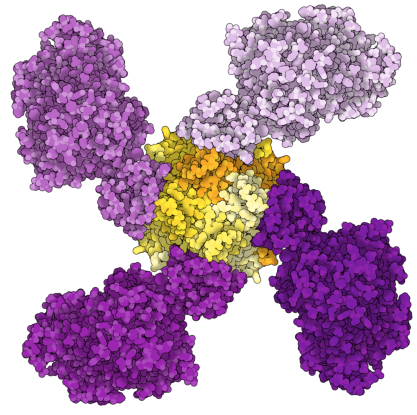
\includegraphics[width=\textwidth]{sur_topdown_propellor.pdf}
	\end{subfigure}
	\hfill
	\begin{subfigure}[t]{0.45\textwidth}
		\caption{}\label{ch1fig:sur_ctd}
		\centering
		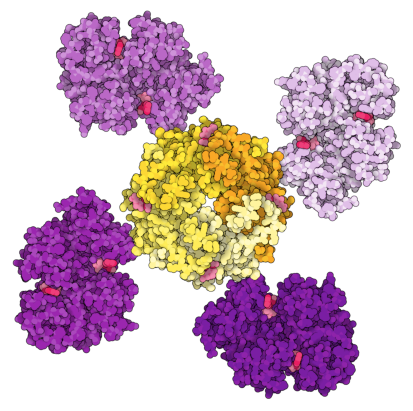
\includegraphics[width=\textwidth]{sur_topdown_ctd_propellor.pdf}
	\end{subfigure}
	\caption[K\textsubscript{ATP} architecture and nucleotide regulation]{
		\subref{ch1fig:katp_cartoon} Membrane topology of the K\textsubscript{ATP} channel shown with two Kir6.2 subunits and one SUR1 subunit.
		\subref{ch1fig:sur_topdown} Top-down view of a cryo-EM structure of the K\textsubscript{ATP} channel (PDB \# 6C3P) solved with nucleotides bound at each of the three canonical binding sites.
		Each SUR1 subunit is shown in a shade of purple, and each Kir6.2 subunit is shown in a shade of orange.
		\subref{ch1fig:sur_ctd} The same view of the structure shown to the left, but with the transmembrane domains removed to reveal the cytoplasmic domains of each subunit only.
		The nucleotides bound to the channel are shown in red.
	}
\end{figure}

\section{Fluorescence methods in ion channel research}

\subsection{Fluorescence as a tool}

\subsection{Forster resonance energy transfer}

\subsection{Unnatural amino acid incorporation}

\section{Functional modelling of ion channels}

\subsection{Why?}

\subsection{A model that fits}
